\documentclass{beamer}

\usepackage[british]{babel}
\usepackage{graphicx,hyperref,ru,url,multicol}
\graphicspath{{images/}}

% The title of the presentation:
%  - first a short version which is visible at the bottom of each slide;
%  - second the full title shown on the title slide;
\title[Towards Embedded Systems]{Towards Embedded Systems}

% Optional: a subtitle to be dispalyed on the title slide
\subtitle{Motivational Role of Free Software }

% The author(s) of the presentation:
%  - again first a short version to be displayed at the bottom;
%  - next the full list of authors, which may include contact information;
\author[Mojtaba Barzegari]{
 Mojtaba Barzegari \\\medskip
  {\small \url{}} \\ 
  {\small \url{mbarzegary@msn.com}}}

% The institute:
%  - to start the name of the university as displayed on the top of each slide
%    this can be adjusted such that you can also create a Dutch version
%  - next the institute information as displayed on the title slide
\institute[Tehran Software Freedom Day]{  }

% Add a date and possibly the name of the event to the slides
%  - again first a short version to be shown at the bottom of each slide
%  - second the full date and event name for the title slide
\date[9/29/2016]
{
  Software Freedom Day\\
  Sharif University of Technology \\
  29th September 2016
}

\begin{document}

\begin{frame}
  \titlepage
\end{frame}

\begin{frame}
  \frametitle{Outline}
 \tableofcontents
\end{frame}

% Section titles are shown in at the top of the slides with the current section 
% highlighted. Note that the number of sections determines the size of the top 
% bar, and hence the university name and logo. If you do not add any sections 
% they will not be visible.

\section{Free Software: a Prison Break}

\begin{frame}
  \frametitle{Free Software: a Prison Break}

  \begin{itemize}
    \item Free Software: Four Essential Freedoms
    \item A bit about History
    \item GNU/Linux
  \end{itemize}
  
  \centering
  
\includegraphics[width=2.5cm]{tux_sc}
  
\end{frame}




\begin{frame}
  \frametitle{Free Software: Four Essential Freedoms}

  \begin{itemize}
    \item
         A program is considered free when its license offers to all its
users the following four freedoms
\begin{itemize}
    \item 
Freedom to \textbf{run} the software for \textbf{any purpose}
\item Freedom to \textbf{study} the software and to \textbf{change} it
\item Freedom to \textbf{redistribute} copies
\item Freedom to \textbf{distribute} copies of \textbf{modified versions}
\end{itemize}
\item These freedoms are granted for both commercial and
non-commercial use
\item They imply the availability of source code, software can be
modified and distributed to customers
\item \textbf{Good match for embedded systems!}
  \end{itemize}
  
\end{frame}



\begin{frame}
  \frametitle{A bit about History}
  
    \begin{itemize}
        \item \textbf{1983}, Richard Stallman, \textbf{GNU} project and the free software
concept. Beginning of the development of gcc, gdb, glibc and
other important tools
\item \textbf{1991}, Linus Torvalds, \textbf{Linux kernel} project, a Unix-like
operating system kernel. Together with GNU software and
many other open-source components: a completely free
operating system, \textbf{GNU/Linux}
\item \textbf{1995}, Linux is more and more popular on server systems
\item \textbf{2000}, Linux is more and more popular on embedded
systems
\item \textbf{2008}, Linux is more and more popular on mobile devices
\item \textbf{2010}, Linux is more and more popular on phones
    \end{itemize}
  
  
\end{frame}



\begin{frame}
  \frametitle{GNU/Linux}
  
  \begin{block}{Richard Stallman}
   What you guys are referring to as Linux, is in fact, GNU/Linux, or as I've recently taken to calling it, GNU plus Linux. Linux is not an operating system unto itself, but rather another free component of a fully functioning GNU system made useful by the GNU corelibs, shell utilities and vital system components comprising a full OS as defined by POSIX.
  \end{block}
  
    \centering
  
\includegraphics[width=8cm]{controversy}
  
\end{frame}


\section{Play Your Notes: Embedded Systems}

\begin{frame}
  \frametitle{Play Your Notes: Embedded Systems}
  
  \begin{itemize}
      \item What is an Embedded System?
      \item What makes Embedded Systems different?
      \item Embedded Systems Complexity
      \item To Be or Not to Be, That is the Question
  \end{itemize}
  
    \centering
  
\includegraphics[width=3cm]{tux_bass}

\end{frame}


\begin{frame}{What is an Embedded System?}

    \begin{block}{}
        An embedded system is a computer system with a \textbf{dedicated function} within a larger mechanical or electrical system, often with real-time computing constraints. It is \textbf{embedded} as part of a complete device often including hardware and mechanical parts. Embedded systems control many devices in common use today
    \end{block}
    
        \centering
  
\includegraphics[width=2.5cm]{tux_worker}
    
    
\end{frame}


\begin{frame}
  \frametitle{What makes Embedded Systems different?}
  
  \begin{itemize}
      \item Real-time operation
        \item Size
        \item Cost
        \item Time
        \item Reliability
        \item Safety
        \item Energy
        \item Security
  \end{itemize}
\end{frame}

\begin{frame}
  \frametitle{Embedded Systems Complexity}
  
  \begin{block}{Moore's Law (Second edition)}
    The observation made in 1975 by Gordon Moore, co-founder of Intel, that the number of transistors per square inch on integrated circuits had doubled every double year since the integrated circuit was invented.
  \end{block}
  
      \centering
  
\includegraphics[width=2.5cm]{tux_moore}
  
\end{frame}


\begin{frame}{To Be or Not to Be, That is the Question}
    
    \begin{block}{}
    So, why does your TV run Linux? At frst glance, the function of a TV is simple: it has to display a stream of video on a screen. Why is a complex Unix-like operating system like Linux necessary?
    \end{block}
    
    \\
    \\
    
        \centering
  
\includegraphics[width=3cm]{tux_inside}
    
    
\end{frame}


\section{Digital Electronics and Operating Systems}

\begin{frame}
  \frametitle{Digital Electronics and Operating Systems}
  
  \begin{itemize}
      \item Electronics: Analog and Digital
      \item Enter the Sandman: Microcontroller
      \item Productivity Nightmares: Primary Solutions
      \item Open Source OSes
      \item Linux and Free Software
  \end{itemize}
  
    \centering
  
\includegraphics[width=2.5cm]{tux_dig}  
  
\end{frame}


\begin{frame}{Electronics: Analog and Digital}

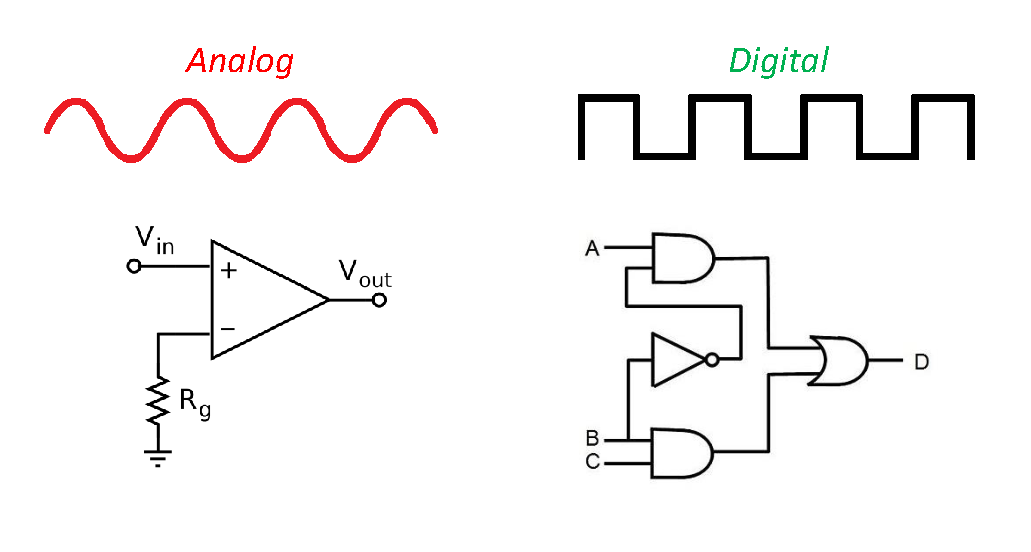
\includegraphics[width=10cm]{AD}

\end{frame}


\begin{frame}{Enter the Sandman: Microcontroller}

\begin{itemize}
    \item 
Gate + Clock $\Rightarrow$ Microprocessor
    \item 
Microprocessor + Peripherals $\Rightarrow$ Microcontroller
    \item 
Microcontroller + CoProcessors $\Rightarrow$ Embedded Processor
\end{itemize}

    \centering
  
\includegraphics[width=2.5cm]{tux_sandman}

\end{frame}


\begin{frame}{Productivity Nightmares: Primary Solutions}
    Serious Challenges:
    \begin{itemize}
        \item Managing Peripherals 
        \item Moore's Law
        \item Programming APIs
        \item Hardware Dependency
    \end{itemize}
    
    Recommended Solutions:
    \begin{itemize}
        \item Open Hardware
            \begin{itemize}
                \item Arduino/Genuino
            \end{itemize}
        \item Open Source Hardware Programming Platforms
        \begin{itemize}
             \item Mbed
        \end{itemize}
        \item Operating System
    \end{itemize}
\end{frame}



\begin{frame}{Open Source OSes}
    
    \begin{itemize}
  
  \item \textbf{FreeRTOS}
  \item \textbf{RIOT}
  \item Contiki
  \item TinyOS
  \item OpenWSN
  \item Zephyr
  \item \textbf{GNU/Linux}
  
    \end{itemize}
    
\end{frame}


\begin{frame}{Linux and Free Software}

Advantages of Linux and Free Software for embedded systems:

\begin{itemize}
    \item Re-using components
    \item Low cost
    \item Full control
    \item Quality
    \item Easy testing of new features
    \item Community support
\end{itemize}
    
\end{frame}



\begin{frame}{Re-using components}
    \begin{itemize}
        \item  The key advantage of Linux and open-source in embedded
systems is the \textbf{ability to re-use components}
\item The open-source ecosystem \textbf{already provides} many
components for standard features, from hardware support to
network protocols, going through multimedia, graphic,
cryptographic libraries, etc.
\item As soon as a hardware device, or a protocol, or a feature is
wide-spread enough, high chance of having open-source
components that support it.
\item Allows to \textbf{quickly design and develop} complicated products,
\textbf{based on existing components}.
\item No-one should re-develop yet another operating system kernel,
TCP/IP stack, USB stack or another graphical toolkit library.
\item Allows to \textbf{focus on the added value of your product}.
    \end{itemize}    
\end{frame}


\begin{frame}{Low cost}
    \begin{itemize}
        \item Free software \textbf{can be duplicated} on as many devices as you
want, \textbf{free of charge}.
\item If your embedded system uses only free software, you can
reduce the \textbf{cost of software licenses to zero}. Even the
development tools are free, unless you choose a commercial
embedded Linux edition.
\item Allows to have a higher budget for the hardware or to
increase the company’s skills and knowledge
    \end{itemize}    
\end{frame}


\begin{frame}{Full control}
    \begin{itemize}
        \item With open-source, you have the source code for all
components in your system
\item Allows \textbf{unlimited modifications, changes, tuning, debugging,
optimization}, for an unlimited period of time
\item Without lock-in or dependency from a third-party vendor
\item To be true, non open-source components must be avoided
when the system is designed and developed
\item Allows to have \textbf{full control over the software part} of your
system
    \end{itemize}    
\end{frame}


\begin{frame}{Quality}
    \begin{itemize}
        \item Many open-source components are \textbf{widely used}, on millions of
systems
\item Usually \textbf{higher quality} than what an in-house development can
produce, or even proprietary vendors
\item Of course, not all open-source components are of good
quality, but most of the widely-used ones are.
\item Allows to \textbf{design your system with high-quality
components} at the foundations
    \end{itemize}    
\end{frame}


\begin{frame}{Easy testing of new features}
    \begin{itemize}
        \item Open-source being freely available, it is \textbf{easy to get a piece of
software and evaluate it}
\item Allows to \textbf{easily study several options} while making a choice
\item Much \textbf{easier than purchasing} and demonstration procedures
needed with most proprietary products
\item Allows to \textbf{easily explore new possibilities} and solutions
    \end{itemize}    
\end{frame}


\begin{frame}{Community support}
    \begin{itemize}
        \item Open-source software components are developed by
communities of developers and users
\item This community can provide a \textbf{high-quality support}: you can
directly contact the main developers of the component you
are using. The likelyhood of getting an answer doesn't depend
what company you work for.
\item Often better than traditional support, but one needs to
understand how the community works to properly use the
community support possibilities
\item Allows to \textbf{speed up the resolution of problems} when
developing your system
    \end{itemize}    
\end{frame}


\begin{frame}{Linux Disadvantages!!!}

\begin{itemize}
    \item
     Linux certainly is a robust and developer-friendly OS
     \item Linux will have many uses in embedded devices, particularly
ones that provide graphically rich user interfaces.
\item
Linux has a disadvantage when compared to other embedded operating systems:
\begin{itemize}
\item Memory footprint
\item It simply will not run on 8 or 16-bit MCUs
\item Real-time operations problem
\end{itemize}
\end{itemize}


        \centering
  
\includegraphics[width=3cm]{tux_weak}


\end{frame}


\section{Real-Time OS: Dream or Reality??}

\begin{frame}
  \frametitle{Real-Time OS: Dream or Reality??}
  
  \centering
  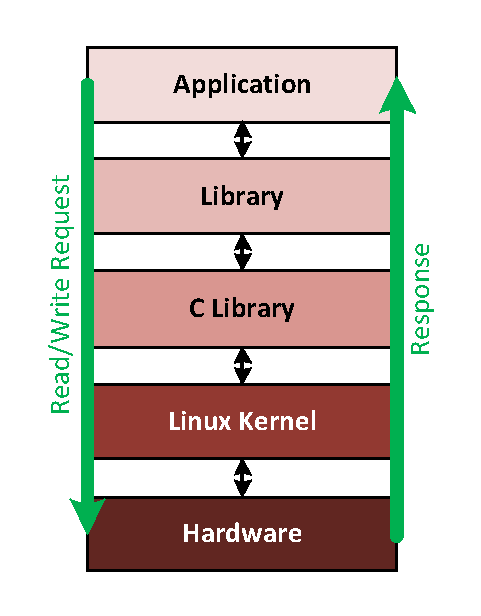
\includegraphics[width=5cm]{RT}
  
\end{frame}

\begin{frame}
  \frametitle{Real-Time OS: Dream or Reality??}

    \textbf{Typical Problems}:
    \begin{itemize}
        \item Controlling Servo Motors
        \item Generating High Frequency Signals
        \item Generating PWM and Duty Cycles
        \item Sampling a Signal (e.g. Audio Signal)
        \item Controlling a Sensitive Robot
        \item Developing Flight Controllers
    \end{itemize}


\end{frame}

\begin{frame}
  \frametitle{Real-Time OS: Dream or Reality??}

    \textbf{Suggested Solutions}:
    

    \begin{enumerate}
        \item 
        Using High-Speed Interfaces
            \begin{itemize}
            \item PCI
            \item Ethernet
            \item USB
            \item RS232
        \end{itemize}
        \item Developing System Drivers
        \item Designing Auxiliary Hardware and Co-Processor
    \end{enumerate}    
    
            \centering
  
\includegraphics[width=3cm]{tux_sound}


\end{frame}
\section{Internet of Things: Domination of Free Software}

\begin{frame}
  \frametitle{Internet of Things: Domination of Free Software}
  
  \begin{itemize}
      \item What is Internet of Things (IoT)?
      \item Things Connected Through Internet
      \item IoT Applications
      \item Top Free and Open Source IoT Projects
      \item Rise of Linux: IoT-ready Hardwares
      \item Beyond the IoT: The Computation Thunderbolt
  \end{itemize}
  
        \centering
  
\includegraphics[width=2.5cm]{tux_dom}

\end{frame}




\begin{frame}
  \frametitle{What is Internet of Things (IoT)?}
  
  \begin{block}{What is IoT?}
  [\textbf{Wikipedia}]: The network of physical objects or things embedded with
electronics, software, sensors, and connectivity to enable objects to exchange
data with the manufacturer, operator and/or other connected devices.
  \end{block}

  \begin{block}{What is IoT?}
  [\textbf{WhatIs}]: A scenario in which objects, animals or people are provided with
unique identifiers and the ability to transfer data over a network without
requiring human-to-human or human-to-computer interaction.
  \end{block}

\end{frame}


\begin{frame}{Things Connected Through Internet}


\includegraphics[width=8cm]{IoT}
    
\end{frame}




\begin{frame}{IoT Applications}

\begin{itemize}
    \item Smart home
\item Wearables
\item Smart City
\item Smart grids
\item Industrial Internet
\item Connected Car
\item Connected Health
\item Smart Retail
\item Smart Supply Chain
\item Smart Farming
\end{itemize}

\end{frame}

\begin{frame}{Top Free and Open Source IoT Projects}
    % https://www.linux.com/news/21-open-source-projects-iot
    \begin{itemize}
        \item AllSeen Alliance (Interoperability framework) 
        \item DeviceHive (Big Data analytics)
        \item DSA (Distributed Services Architecture)
        \item Eclipse IoT (Java-based rules-based routing engine)
        \item Kaa (scalable end-to-end IoT framework )
        \item Macchina.io (Web-enabled, modular and extensible JavaScript and C++ runtime)
        \item Open Connectivity Foundation (IoTivity)
        \item OpenIoT (Java-based connectivity framework)
        \item PlatformIO (Python-based suite for remote data access)
    \end{itemize}
    
\end{frame}

\begin{frame}{Rise of Linux: IoT-ready Hardwares}


\begin{multicols}{2}
    \begin{itemize}
        \item Yocto Project!!!
        \item Raspberry Pi
        \item Intel Edison
        \item Intel Joule
        \item BeagleBone Black
        \item Qualcomm DragonBoard 
        \item MinnowBoard MAX
        \item Orange Pi
    \end{itemize}
\end{multicols}    
      
        \centering
  
\includegraphics[width=7cm]{tux_star}
    
\end{frame}
    
    
    
\begin{frame}{IoT and Linux}

    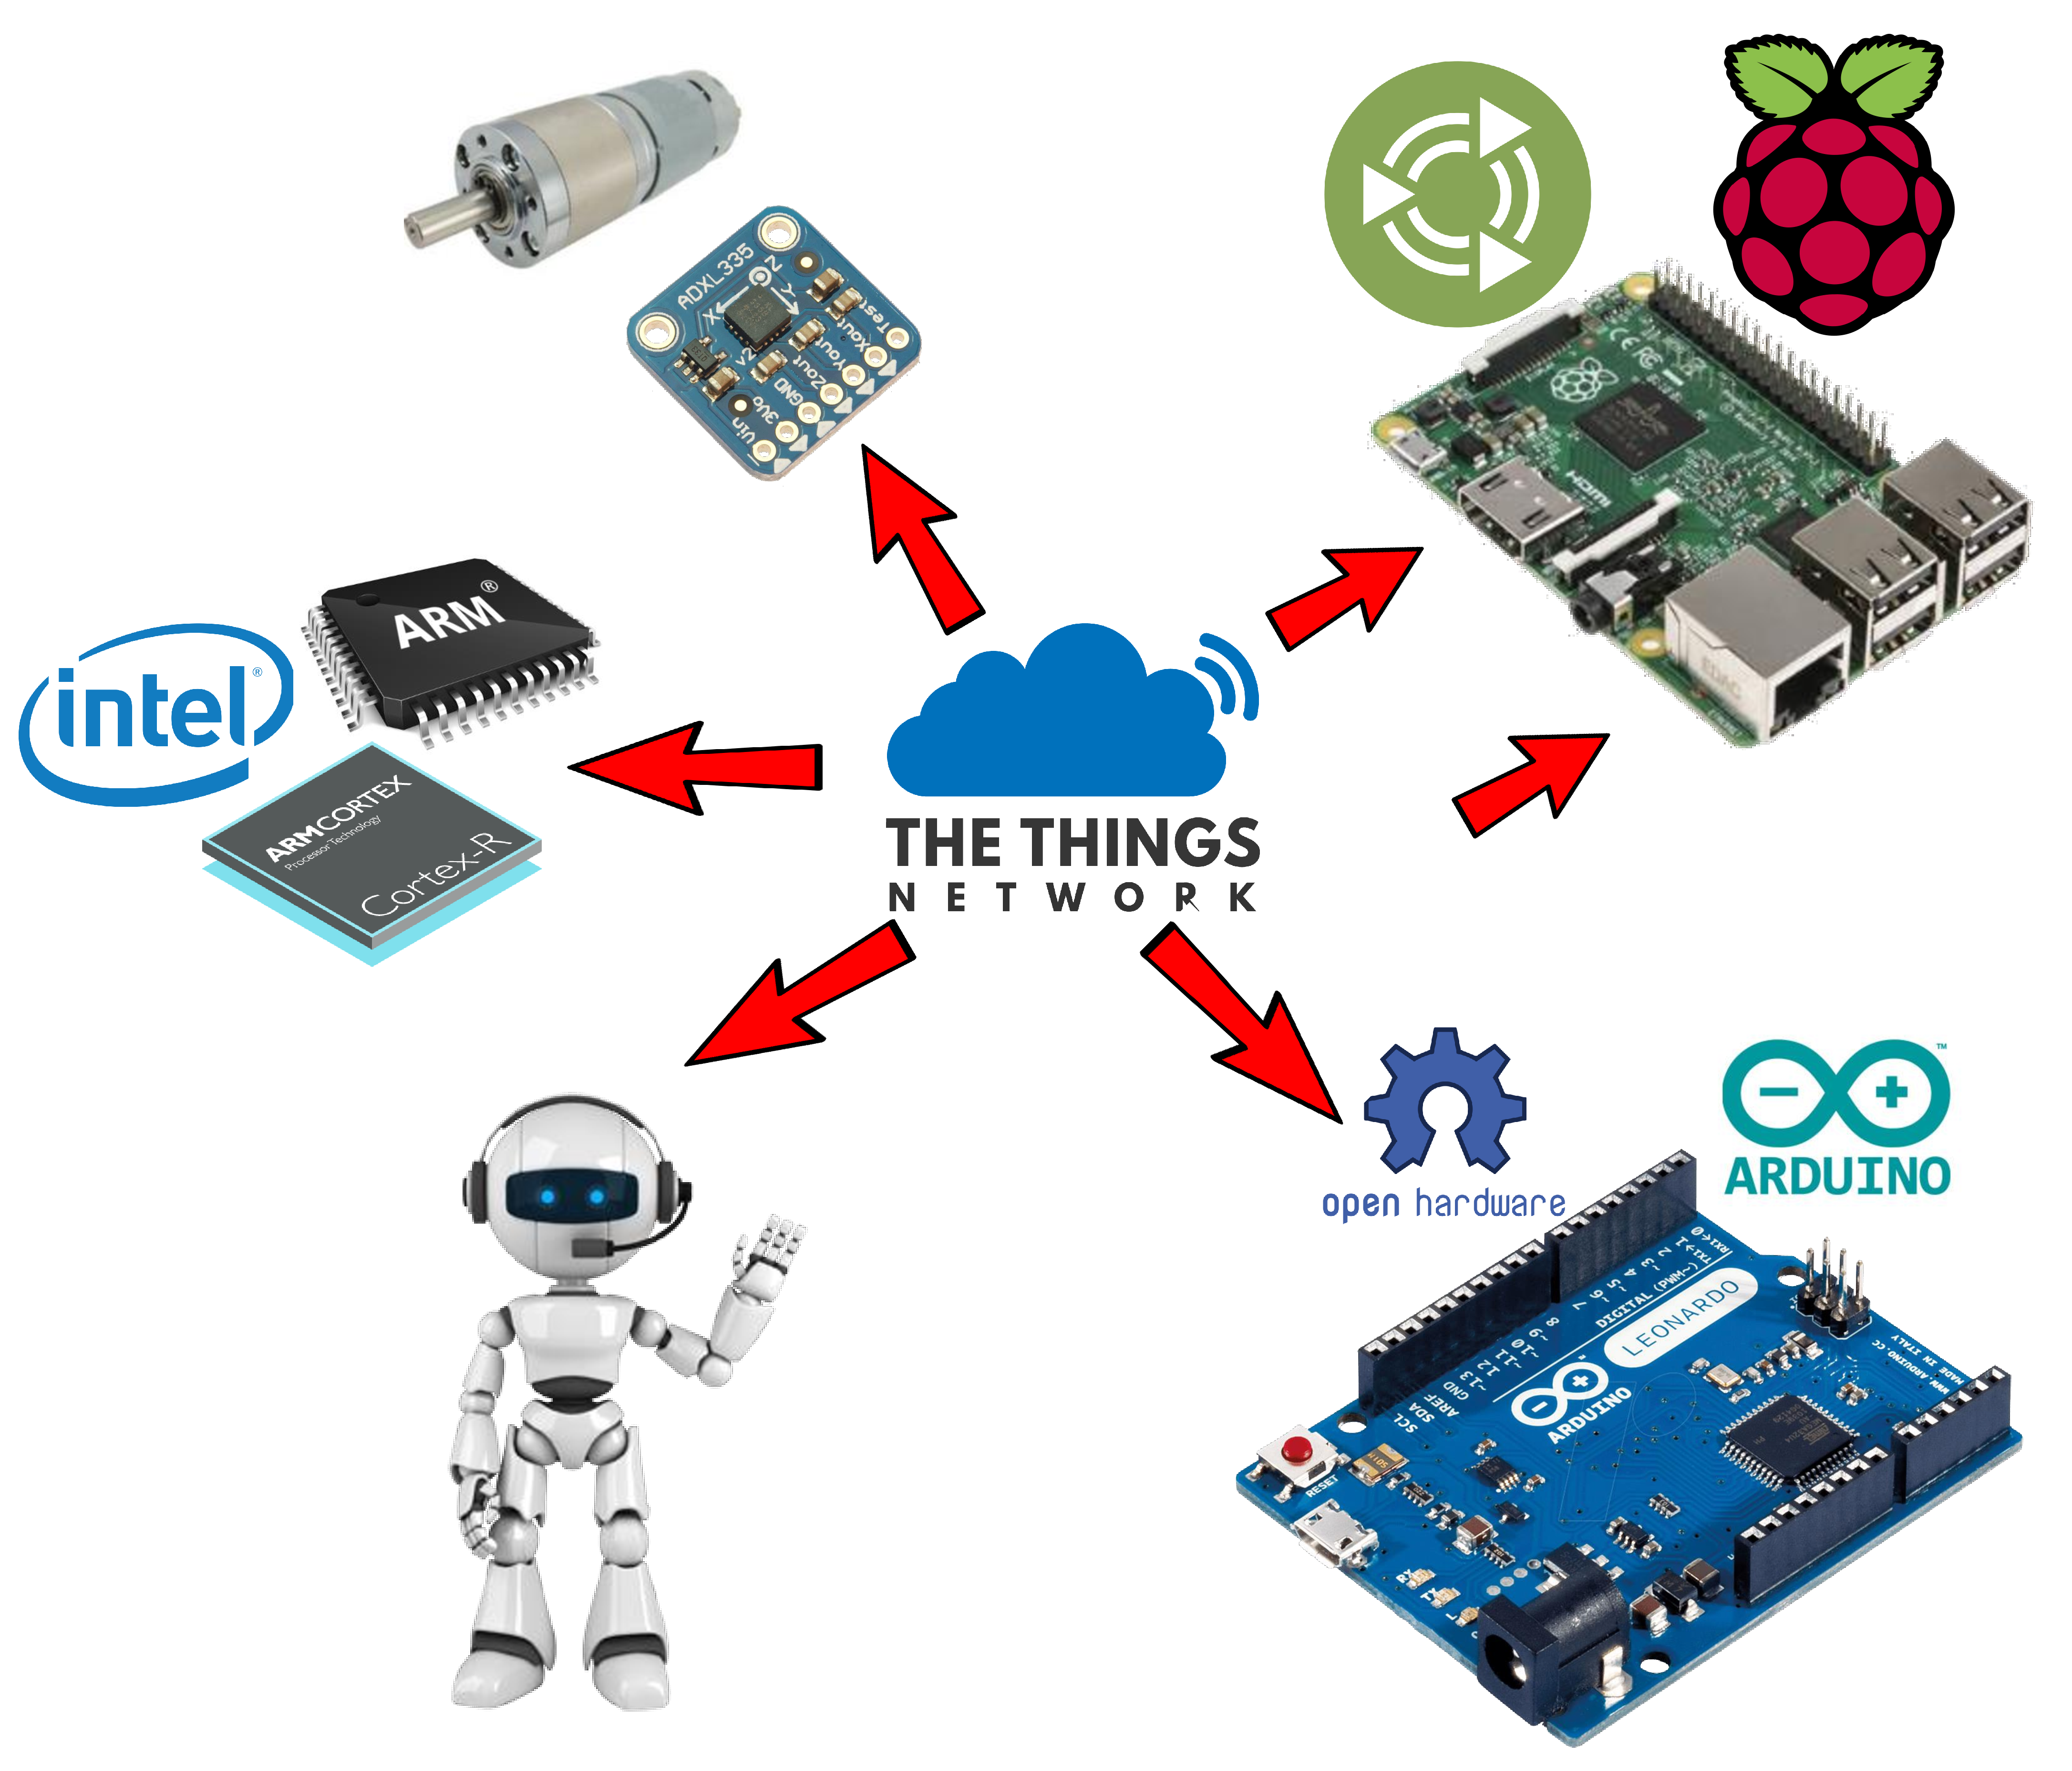
\includegraphics[width=8cm]{IoT_Linux}
    
\end{frame}


\begin{frame}{Raspberry Pi}

\begin{multicols}{2}

    \begin{itemize}
        \item
        \textbf{SoC}: Broadcom BCM2837
        \item
\textbf{CPU}: 4× ARM Cortex-A53, 1.2GHz
\item
\textbf{GPU}: Broadcom VideoCore IV
\item
\textbf{RAM}: 1GB LPDDR2 (900 MHz)
\item
\textbf{Networking}: Ethernet, 2.4GHz 802.11n wireless
\item
\textbf{Bluetooth}: Bluetooth 4.1 Low Energy
\item
\textbf{Storage}: microSD
\item
\textbf{GPIO}: 40-pin header
%\item
%\textbf{Ports}: HDMI, 3.5mm analogue audio-video jack, 4× USB 2.0, Ethernet, Camera Serial Interface (CSI), Display Serial Interface (DSI)
    \end{itemize}
    
    \end{multicols}
    
    \centering
    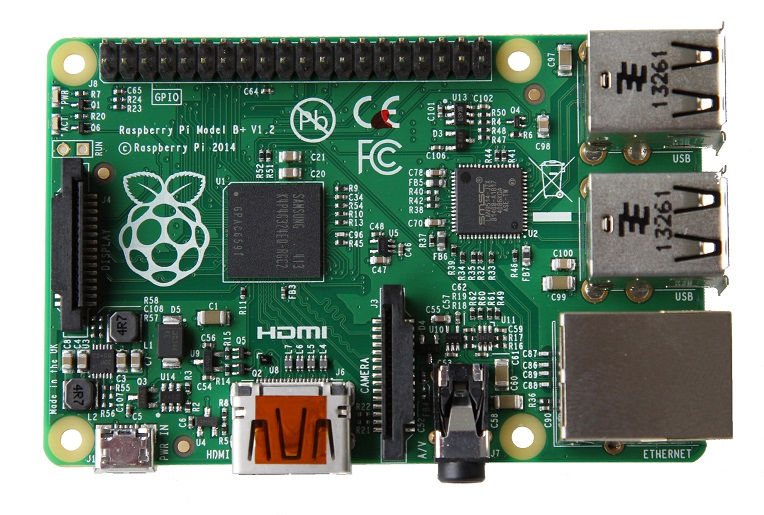
\includegraphics[width=5cm]{rpi}
    
\end{frame}



\begin{frame}{Intel Edison}

\begin{multicols}{2}

\footnotesize
\begin{itemize}
    \item
    \textbf{CPU}: Dual-core Intel Atom @500 MHz
    \item
\textbf{RAM}: 1 GB LPDDR3 
\item
\textbf{Storage}: 4 GB eMMC + micro SD card connector
\item
\textbf{Connectivity}:  Dual band Wi-Fi and Bluetooth 4.0
\item
\textbf{USB}: 1x micro USB connector
\item
\textbf{I/Os}:
\footnotesize
\begin{itemize}
    \item
2x UART  
\item
2x I2C 
\item
1x SPI with 2 chip selects
\item
1x I2S
\item
12x GPIO including 4 capable of PWM output
\end{itemize}
\end{itemize}

\end{multicols}

\centering

\includegraphics[width=3.5cm]{edison}

\end{frame}




\begin{frame}{Intel Joule}

\begin{itemize}
    \item
    \textbf{CPU}: Intel Atom T5700 64-bit quad-core @1.7GHz/2.4GHz
    \item
\textbf{RAM}: 4GB LPDDR4 RAM
\item
\textbf{GPU}: Intel HD Graphics with 4K video capture and display
\item
\textbf{Storage}: 16GB eMMC memory
\item
\textbf{Connectivity}: 802.11ac Wi-Fi with MIMO and Bluetooth 4.1
\end{itemize}

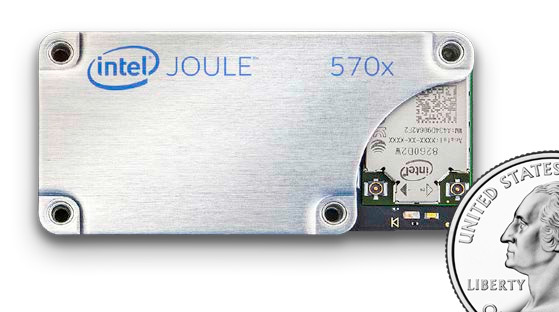
\includegraphics[width=5cm]{joule}


\end{frame}



\begin{frame}{Beyond the IoT: The Computation Thunderbolt }

These devices can be utilized in standalone computations:
\begin{itemize}
    \item Speech Recognition
    \item Machine Learning
    \item Image Processing
    \item Grid Computing
    \item Video Encoding/Decoding
\end{itemize}


\end{frame}
\section{}

\begin{frame}

\frametitle{Conclusion}

    Why Reinvent The Wheel When You Don't Have To???
    
     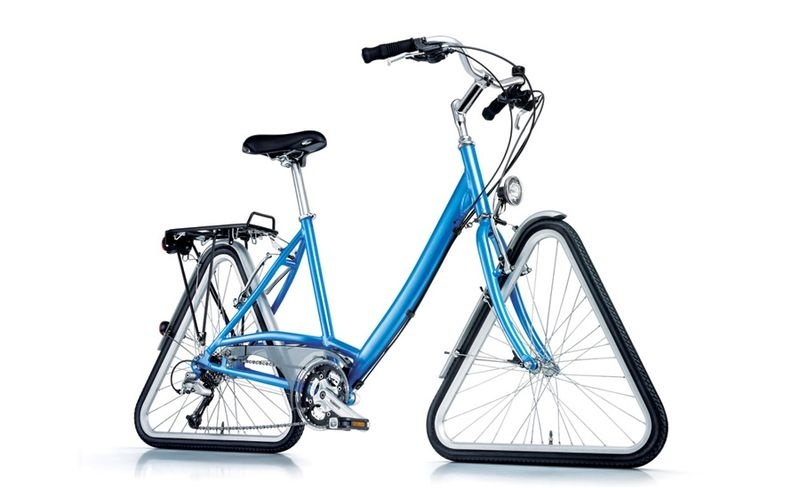
\includegraphics[width=8cm]{wheel}
  
\end{frame}


\begin{frame}{Thanks for Your Attention}


\centering

\includegraphics[width=4cm]{tux_qa}

\centering
Question \& Answer

\end{frame}



\end{document}